\documentclass[tikz, margin=3mm]{standalone}
\usepackage{amsmath,amsfonts,tikz,fontspec}
\usetikzlibrary{arrows.meta, bending, positioning}

\setmainfont{DejaVu Serif}
\setsansfont{DejaVu Sans}

\newcommand{\mathng}{{\text{\normalfont \textit{ŋ}}}}

\newcommand{\txtop}[1]{\mathop{\mathrm{#1}}\limits}
\newcommand{\argmin}{\txtop{argmin}}
\newcommand{\MSE}{\txtop{MSE}}
\newcommand{\ntos}{\txtop{noise2self}}
\newcommand{\PCA}{\txtop{PCA}}
\newcommand{\kNN}{\txtop{kNN}}
\newcommand{\WAK}{\txtop{WAK}}
\newcommand{\leiden}{\txtop{leiden}}
\newcommand{\rdim}{\txtop{reducedimension}}


\begin{document}


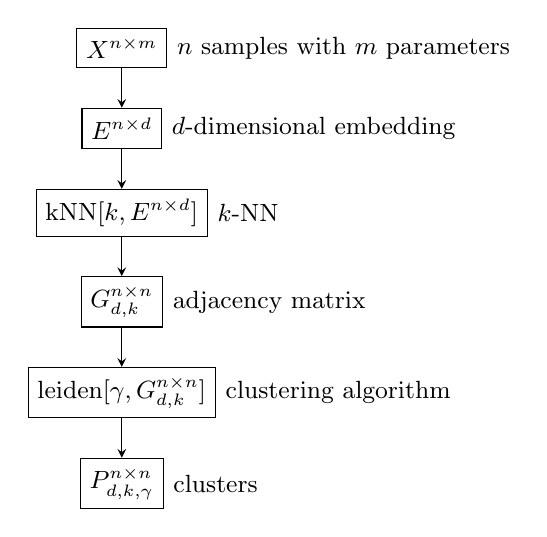
\begin{tikzpicture}[
    node distance = 5mm and 5mm,
    punkt/.style = {rectangle, draw},
    pil/.style = {black, -stealth},
    font=\small
    ]
    %nodes
    \node[punkt,label=right:$n$ samples with $m$ parameters] (X)
            {$X^{n \times m}$} ;
    %\node[punkt,label=right:encoder] (encoder) [below=of X]
    %     {$\theta_e^{m \times \mathng}$} ;
    \node[punkt,label=right:$d$-dimensional embedding] (E)
        [below=of X] {$E^{n \times d}$} ;
    \node[punkt,label=right:$k$-NN] (knn)
        [below=of E]
        {$\kNN[k,E^{n \times d}]$} ;

    \node[punkt,label=right:adjacency matrix] (G) [below=of knn]
            {$G_{d,k}^{n \times n}$};
    \node[punkt,label=right:clustering algorithm] (leiden) [below=of G]
            {$\leiden[\gamma,G_{d,k}^{n \times n}]$};
    \node[punkt,label=right:clusters] (P) [below=of leiden]
        {$P_{d,k,\gamma}^{n \times n}$};

    % edges
    \draw[pil]  (X)     edge    (E)
    (E) edge (knn)
    (knn) edge (G)
    (G) edge (leiden)
    (leiden) edge (P);
\end{tikzpicture}

\end{document}

